\clearpage
\section{Method}
\label{sec:method}

% Initially, we establish a metric based on the concept of the 15-minute city, by evaluating the existing metrics introduced in Section \ref{subsec:accessibility_metrics_based_on_the_15_minute_city} and their shortcomings and then developing our own metric that overcomes these limitations.
Our method is split into three parts.
Initially, we establish a metric based on the concept of the 15-minute city and complement it with a cost metric.
Following this, our focus shifts to finding a fitting routing algorithm to calculate this metric.
We do so by clearly stating the requirements we pose on such an algorithm, explaining why existing algorithms don't meet our criteria, and introducing our own algorithm, designed to meet our requirements. 
The final stage explains how we use our routing algorithm to calculate our metric. 
This integrated approach allows us to thoroughly assess and improve accessibility in urban settings, offering valuable insights for urban planners and decision-makers.

\subsection{Metric}
\label{subsec:metric}

Our metric consists of two dimensions, time and cost.
The time dimension is based on the concept of the 15-minute city and expands on the findings of \shortciteA{olivariAreItalianCities2023}.
The time dimension effectively measures how fast the access to a variety of important amenities is.
To measure this, we categorize amenities into seven essential services: grocery, education, health, banks, parks, sustenance, and shops.
Each category is populated with Points of Interest (POIs) sourced from OSM, providing a comprehensive database of locations.
The POIs are identified by their respective OSM tags.
OSM tags are descriptive labels used to define the attributes and characteristics of geographic features in the OSM database. 
They consist of a key and a value pair, like "amenity=restaurant", which enables categorizing map elements such as roads, buildings, and natural features for accurate and comprehensive mapping.
In our case, we use the OSM tags to identify nodes that represent POIs, like a supermarket or a park.
The categories and their respective tags can be seen in Appendix \ref{app:categories_and_osm_tags}.

The core of our metric is the determination of temporal proximity to these amenities. 
For each category, we calculate the minimum travel time required to reach at least one POI of that category. 
The metric is then defined as the maximum value among these minimal times across all categories and we refer to it as the X-minute city metric, where X represents the maximum value among the minimum travel times.
This approach yields a singular measure that reflects the most significant time distance barrier within an urban area, which effectively captures the least accessible category for any given area.
We think that it is beneficial to focus on the least accessible category, as measuring accessibility in cities by averaging accessibility across all categories can mask disparities categories. 
This ensures that the metric is targeted to areas of greatest need. 
By leveraging this metric, we aim to help city planners to create urban environments that prioritize sustainability, enhance the well-being of residents, and reduce dependency on vehicular transport, thus contributing to the broader goals of efficient urban planning and improved quality of urban life.

% --- comparison to NEXI
Our metric presents several advantages compared to the NEXI-minutes and NEXI-global, as outlined by \shortciteA{olivariAreItalianCities2023}.
Firstly, unlike the NEXI-minutes which calculates separate metrics for each of seven categories, our metric evaluates all categories together. 
This unified approach makes it more straightforward and easier to understand. 
In contrast, while NEXI-global also considers all categories in one assessment, it converts the results into a 0-100 score. 
This percentage system can obscure the real value of the data, making it more difficult to interpret.

Moreover, the NEXI-global's practice of assigning different weights to each category complicates its analysis. 
Our metric, by focusing on the lowest-performing category across all areas, simplifies the understanding and highlights where improvement is most needed. 
This method prevents the dominance of stronger areas over weaker ones, ensuring a more balanced and fair evaluation of urban development. 

% --- cost
In addition to the time dimension, we also incorporate a cost dimension into our metric.
As, we want to incorporate more modes than just walking, some of which may have a monetary cost associated with them, we need to consider the cost of the trip.
We recognize that time and cost are measures of different units and cannot be combined in a sensible way.
Therefore, we draw upon the notion of Pareto optimality to create a multi-objective metric that considers both time and cost.
We define a Pareto set as a set of tuples, where each tuple contains a time value and a cost value.
A tuple can be considered the time that is needed to reach all categories given the cost value.
The Pareto set will allow answering questions in the form of "What is fastest time I can reach all categories given a certain cost?" or "What is the lowest cost I need to pay to reach all categories given a certain time?".

% ---- START section about alternative modes
% explain different modes - maybe(?) this belongs to related work
Traditionally, the 15-minute city concept is applied to walking and or cycling and ignores other modes of transport.
Some researchers, in the context of location-based metrics, even go as far to only calculate the bee-line distance to the nearest amenity and ignore the street network altogether \shortcite{gastnerOptimalDesignSpatial2006}, while most only consider walking \shortcite{olivariAreItalianCities2023, nicolettiDisadvantagedCommunitiesHave2023}.
We, however, believe that to accurately determine the accessibility of a city, all modes of transport must be considered, and the routing needs to be as realistic as possible.
Therefore, we continue with the discussion of requirements we pose on our routing algorithm next.


\subsection{Routing Algorithm}
\label{subs:routing_algorithm}

In this section we will first define the requirements we pose on our routing algorithm and explain why existing algorithms don't meet our criteria.
Next, we will explain our algorithm in detail, which is based on a modular approach, where one module represents one mode of transport.
After that we will explain the modules we use in our experiments, which are either based on MLC or McRAPTOR.
Lastly, we will explain some enhancements we made to MLC and McRAPTOR in order to support multi-objective optimization with dynamic pricing schemes.

\subsubsection{Requirements}
\label{subsubsec:requirements}

% requirements on routing algorithm
% - unrestricted
% - multi-modal (must incorporate scheduled networks (public transfer) and an arbitrary number of other unscheduled networks)
% - multi-objective (must be able to incorporate an arbitrary amount of objectives), whose values update based on the previous values and the current edge (either unscheduled network edge or trip between two stops)
% - inter-modal (the different transport modes may be sequenced in any order (not just bicycles for start and end)
% - modular (the algorithm should be easily adaptable to different modes of transport and the combination of different modes of transport)

In order to fully grasp the potential of the combination of the sustainable modes of transport, we require our routing algorithm to be \textbf{multi-modal}, \textbf{multi-objective}, \textbf{unrestricted inter-modal}, and \textbf{modular}.

\textbf{Multi-modal} means that our routing algorithms allows multiple modes of transport, including scheduled transport systems, like public transfer and an arbitrary number of unscheduled transport systems, like walking, cycling and driving.
In addition, we require that free-floating vehicle sharing systems are incorporated realistically.
That means, that our routing algorithm must consider that switching to a free-floating vehicle is possible at any location, where a free-floating vehicle is available and parking a free-floating vehicle is possible anywhere where it's allowed.
% note: this extra excludes MCR

\textbf{Multi-objective} means that our algorithm must find all pareto optimal journeys according to an arbitrary amount of objectives.
The algorithm must provide the possibility to update the values of any objective whenever a \textit{movement} occurs.
We define a movement either as an edge traversal in an unscheduled network or a step in the route traversal during McRAPTOR.
In the case of an edge traversal the new objective must be a function of the old objective and the edge weights, formally: \(l' = f(l, w(e))\), where \(l\) and \(l'\) are the old and new labels, respectively, and \(w(e)\) are the weights of the edge that is traversed.
In the case of an update during a step of the route traversal, the new objective must be a function of the old objective (to be continued).

\textbf{Inter-modal} means that the different transport modes may be sequenced in any order.
For example, when considering walking, cycling through a bicycle sharing system and public transport, the algorithm needs to consider journeys with bicycle rides between two consecutive public transport trips.

\textbf{Unrestricted} means that the algorithm fully searches the unscheduled network graphs, and does not pose restrictions like a maximum of 10 minutes walking distance.

\textbf{Modular} means that the algorithm should be easily adaptable to different modes of transport.
It should be possible to easily add, remove or chain different modes of transport.


% handled:
% dijkstra, mlc, raptor, ultra, mcraptor, mcr
% relate to other algorithms
Both Dijkstra and MLC are not considered due to their impractical runtime.
Furthermore, the need for multi-objective solutions excludes Dijkstra, RAPTOR, and ULTRA.
The requirement for unrestricted inter-modal travel makes RAPTOR and McRAPTOR unsuitable in practical scenarios.
To explain this, let's examine a straightforward example.
Consider the OSM graph of the key regions in Cologne, which comprises 125,176 nodes and 142,074 edges.
For RAPTOR to compute a transitively closed graph, it requires calculating the walking distance between each node.
This computation would yield \(125,176^2 = 15,669,030,976\) edges, a number vastly greater than the original 142,074 edges.
While MCR does support multi-objective solutions with unrestricted inter-modal transfers, it doesn't fully encapsulate the multi-modal concept we require.
Although it theoretically permits various modes of unscheduled transport, it is primarily tailored for station-based vehicle sharing systems.
Our focus, however, is on the increasingly prevalent free-floating systems.
In MCR, unscheduled networks are contracted, leading to the removal of certain nodes.
If an optimal route requires a mode change at a deleted node, MCR will be unable to identify that path.
As a result, MCR is not a viable option for our needs.
Also note, that none of the algorithms mentioned so far are modular.

\subsubsection{Scaffolding Algorithm}
\label{subsubsec:algorithm}

% introduction modules
As said, our algorithm should be easily adaptable to different modes of transport, therefore, we formulate it in a modular fashion.
The algorithm described next presents a scaffolding that needs to be augmented by different modules, where a module represents a specific mode of transport and running a module may be seen as fully exploring the network through this mode of transport.
One module, for example, would be walking, and running the walking module would mean to traverse the whole walking graph given the current state of bags.

% explanation of bags & need for common network 
A module always takes bags as an input and returns bags as an output.
As explained in Section \ref{sec:related_work} a bag is a set of labels, that are Pareto optimal with respect to the objectives.
In addition, in our work, a bag is associated with a node on some network.
For the bags that are the input and output of the modules, we further require that they are associated with the same network.
This is necessary in order to merge the bags of different modules.
The most reasonable choice for the common network is the walking graph, as this has a real-world interpretation, because walking between different modes of transport is very common.

% example of running a module
To further explain how running a module looks like, consider the example of calling the walking module on the starting bags, which are a set of bags, where every bag is empty, except for the one of the starting node, where exactly one label is present that contains the starting time and zero costs.
The output would be a set of bags, where each node's bag contains exactly one label where the time would be equal to the time it takes to walk to the node and the cost would be zero, as walking never costs anything.

% algorithm
The scaffolding algorithm is shown in Figure \ref{fig:modular_routing_algorithm}.
The algorithm takes a start node and time as input and returns bags.
First it creates the starting bags described above from the start node and the start time.
Next, it runs the initial modules given by the initial module matrix.

A module matrix is an irregular matrix of modules.
To run the module matrix, first the modules of the first row are run in parallel.
Their respective outputs are then merged into a single set of bags.
After that the second row is run and so on and so forth.
This process is also described in Figure \ref{fig:modular_routing_algorithm}.

After the initial modules are run, the same is done for the repeating modules for the specified number of times.
By convention, we count each iteration of the repeating modules as one trip.

\begin{figure}
    \centering
    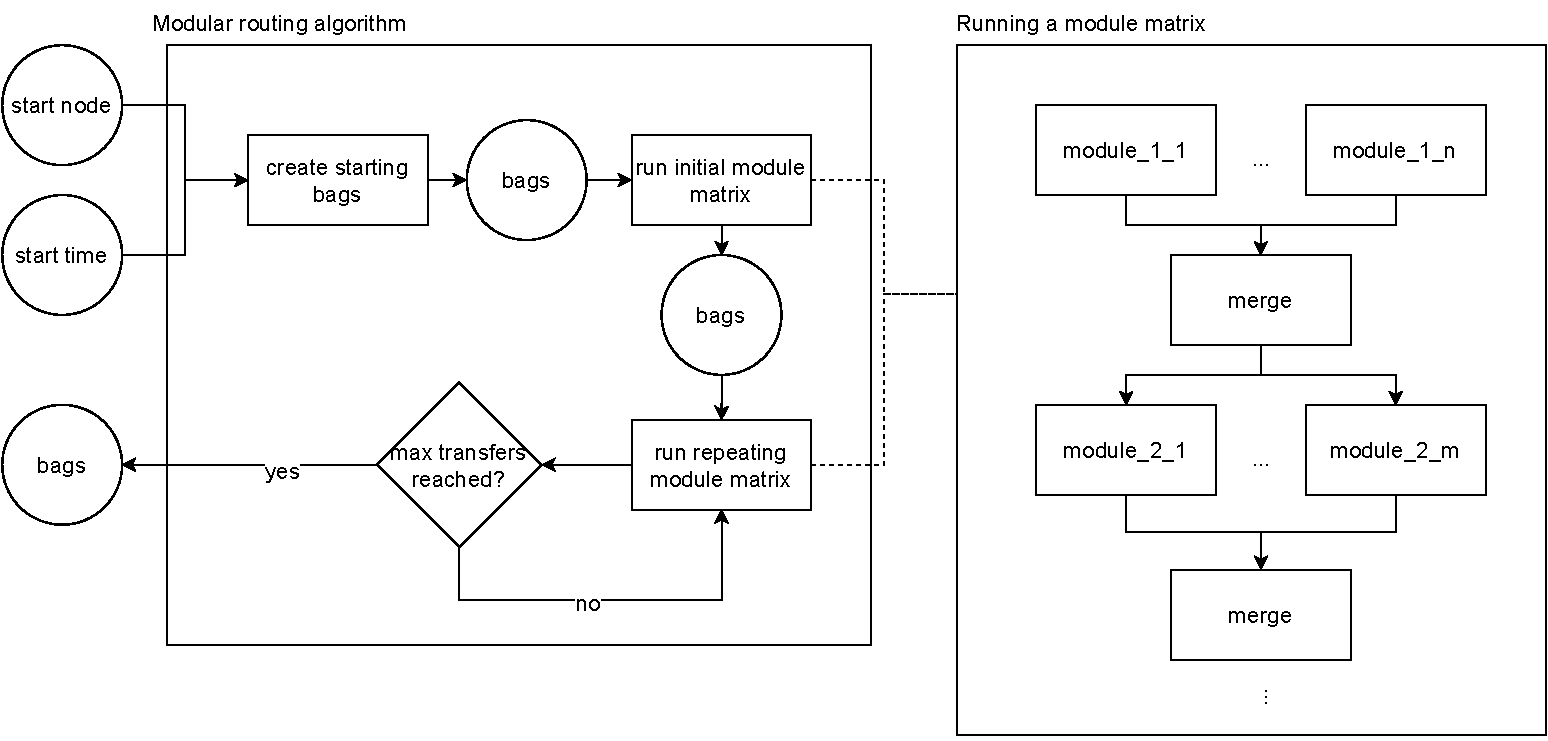
\includegraphics[scale=0.40]{Figures/method/modular_routing_algorithm}
    \caption{Modular Routing Algorithm}
    \label{fig:modular_routing_algorithm}
\end{figure}


\subsubsection{Modules}
\label{subsubsec:modules}

In our experiments, we categorize four modules into two types: unscheduled and scheduled. 
The unscheduled modules consist of walking, free-floating vehicle sharing, and personal vehicle use and are based on MLC, while the scheduled module is public transport, which is based on McRAPTOR.

Walking is the simplest unscheduled module, it simply consists of running MLC on the walking graph.
The edges of the walking graph should contain the time it takes to traverse them by foot and should not have any monetary cost associated with them.

The free-floating vehicle sharing module is a bit more complex.
Before running MLC on the respective vehicle graph, the module filters our all bags that are located at a node where no free-floating vehicle is available.
In addition, the vehicle graph is augmented with a walking graph. 
This means that at nodes in the vehicle graph, where it is allowed to park the vehicle, there is an edge to the closest node in the walking graph.
This augmentation is necessary, as the output bags of the free-floating vehicle sharing module need to be associated with nodes in the walking graph, as it is the common network.
The module may also define cost depending on the time spent on the trip.

For the personal vehicle module, we assume that there is only one personal vehicle and that it is located at the starting node.
Therefore, the module filters out all bags that are not located at the starting node.
Obviously, this module is only useful for the first trip, or more precisely, the module should only be used in the first row of the initial module matrix.
After that MLC is run on the vehicle graph again augmented with the walking graph.
As this module is also based on MLC, it may define costs just like the free-floating vehicle sharing module.

In comparison to the unscheduled modules, the public transport module does not use MLC, but McRAPTOR.
As a first step the module filters out all bags that are associated with a node that is not near a stop in the public transport system.
Next, the module performs a single iteration of McRAPTOR, which represents a single trip within the public transport system.
Last, the resulting bags have to be associated with nodes in the walking network again.
To do so, the modules simply use the node that is closest to the coordinates of the public transport stop.
Similarly to the free-floating vehicle sharing and personal vehicle module, the public transport module may define costs.
The cost may depend on the number of stops that are traversed during the trip.

\subsubsection{Merging}
\label{subsubsec:merging}

The merging of bags after running multiple modules in parallel is quite simply.
Each bag represents a set of Pareto optimal labels and each bag is associated with a node.
We therefore merge bag-wise.
We differentiate between two cases:
\begin{enumerate}
    \item There is only one bag associated with a node.
    \item There are multiple bags associated with the same node.
\end{enumerate}
In the first case, we simply put the bag into the output bags.
In the second case, we create a new bag that contains all labels of all bags associated with the node, which might break the Pareto optimality of the labels.
Therefore, to restore the Pareto optimality of the labels, we remove all labels that are dominated by another label.

\subsubsection{Enhanced MLC \& McRAPTOR}
\label{subsubsec:enhanced_mlc_and_mcraptor}

To address the multi-objective optimization involving both time and monetary cost, we introduce enhancements to MLC and McRAPTOR. 
The standard versions of MLC and McRAPTOR do not adequately capture dynamic pricing models, which is necessary to realistically represent monetary costs.

% \paragraph{Challenges in the Original Algorithms} 
The original MLC associates a fixed cost with an edge, which cannot represent variable pricing, such as a bike-sharing tariff that costs 1\euro per 15-minute increment. 
Labels are only updated by adding the cost of a given edge to the label's values.
Similarly, McRAPTOR updates the labels at each stop during route traversal only based on the information of the current trip and stop. 
With this McRAPTOR is unable to represent a pricing scheme that varies with the number of stops, like the one used by the Cologne Transport Authority.
Our proposed modifications involve the use of 'hidden values' within the labels that are used by these algorithms. 
These hidden values carry additional information which is not considered when comparing labels, but that may be used to update cost dynamically.

In the case of MLC, the hidden values may be updated along any edge, just like the regular values of the label.
A hidden value, may carry information on how long the current trip with the shared vehicle is.
We then additionally allow defining a function that updates while traversing an edge and may use the values and hidden values both before and after the traversal to do the update.
With this functionality it is easy to increment the cost by 1\euro every time the time spent on the trip exceeds the 15-minute interval.

Similarly, the hidden values may be updated during McRAPTOR after every iteration of a stop.
We can, therefore, store how many stops the current trip already traversed and if that number exceeds four, we can easily increase the price from 2.20\euro to 3.20\euro.

Additionally, as the concept of hidden values isn't specific to MLC or McRAPTOR, the hidden values can be transferred across iterations and modules.
To understand the benefit, again consider the example of the pricing of the Cologne Transport Authority.
The ticket that costs 3.20euro allows traveling any number of trips within Cologne, no matter if it is necessary to change to a different trip.
Therefore, if we were to first travel two stations with one trip and then get out to catch another trip that consists of five stops, we would still have the information that we already commuted two stops.
Therefore, we can charge 3.20euro, instead of charging 2.20euro two times, which is more realistic.
These enhanced versions of MLC and McRAPTOR are used in our modules, so that we can use the more realistic dynamic pricing schemes.

While running our experiment, we see that MLC based modules present a significant computational bottleneck.
We observe that in order to calculate our metric, we don't actually need to have the labels of every single node, but only of those, that impact the X-minute city and time Pareto front.
We therefore introduce a runtime optimization into MLC, which eliminates some bags from being processed that are guaranteed to not impact the Pareto front.
While iterating the unprocessed bags in MLC, we keep track of the minimum time required to reach a POI node of each category for each cost value.
If we encounter a bag whose time and cost values are both greater than the minimum time and cost values for all categories, we can safely discard this bag, as it will not impact the Pareto front.


\subsubsection{Example}
\label{subsubsec:example}

To illustrate our algorithm, we will now go through an example step by step.
The module configuration we use in our example represents travelling by free-floating vehicle sharing, public transport and walking.
The initial module matrix just contains the walking module, in order to initially reach the free-floating vehicles, as well as, the public transport stops.
The repeating module matrix consists of first the free-floating vehicle sharing module and the public transport module in parallel and then the walking module.
It can be seen in Figure \ref{fig:example_module_matrix}.


\begin{figure}[ht]
\centering
\[
\begin{pmatrix}
\text{free-floating vehicle} & \text{public transport} \\
\text{sharing module} & \text{module} \\
\\
\text{walking} & \\
\end{pmatrix}
\]
\caption{Example Repeating Module Matrix}
\label{fig:example_module_matrix}
\end{figure}

In our example, we assume that both public transport and vehicle sharing has some form of cost associated with it.
The objective is to minimize arrival time and cost.
We also only consider a maximum of two trips.

First we run the initial modules, which in our case is just the walking module on the starting bags.
As the starting bags only consist of one non-empty bag at the starting node with exactly one label, running MLC on the walking graph is equivalent to running Dijkstra's algorithm.
In the real-world this represents walking to all nodes in the walking network from the start node.
Note, that after the initial walking module all bags only contain exactly one label, as the cost to go anywhere by foot is zero.

Next the modules of the first row of the repeating matrix are run.
In the real-world this means that after an initial walk the traveler would either drive with a free-floating vehicle starting from a location where one is available or commute by public transport starting from one stop.
For public transport one could imagine that we commute with all possible trips from all stops and update the bags of the stops along each route accordingly.
After running these modules and merging their result bags, each bag may contain more than one label, as public transport and driving with a vehicle may be faster than walking, but also cost money.
It may even be that some bags contain three different labels, if, for example, driving with a vehicle is the fastest but also costs the most money and commuting by public transport is faster than walking.
The next step consists of running the second row of the repeating module matrix, which in our case is the walking module again.
Running the walking module in the repeating module matrix is important in order to reach nearby POIs after commuting through the public transport system.
After that the repeating module matrix is run again, as we consider a maximum of two trips.
The result of the second run of the repeating module matrix is our final result.



\subsection{Integrated Accessibility Analysis Routine}
\label{subsec:combining}

We embed the routing algorithm described in Section \ref{subsec:routing_algorithms} in our accessibility analysis routine to compute the metric described in Section \ref{subsec:metric}.
Our accessibility analysis routine consists of three parts: the input routine, the main routine and the metrics routine.

% Input routine
\begin{figure}
    \centering
    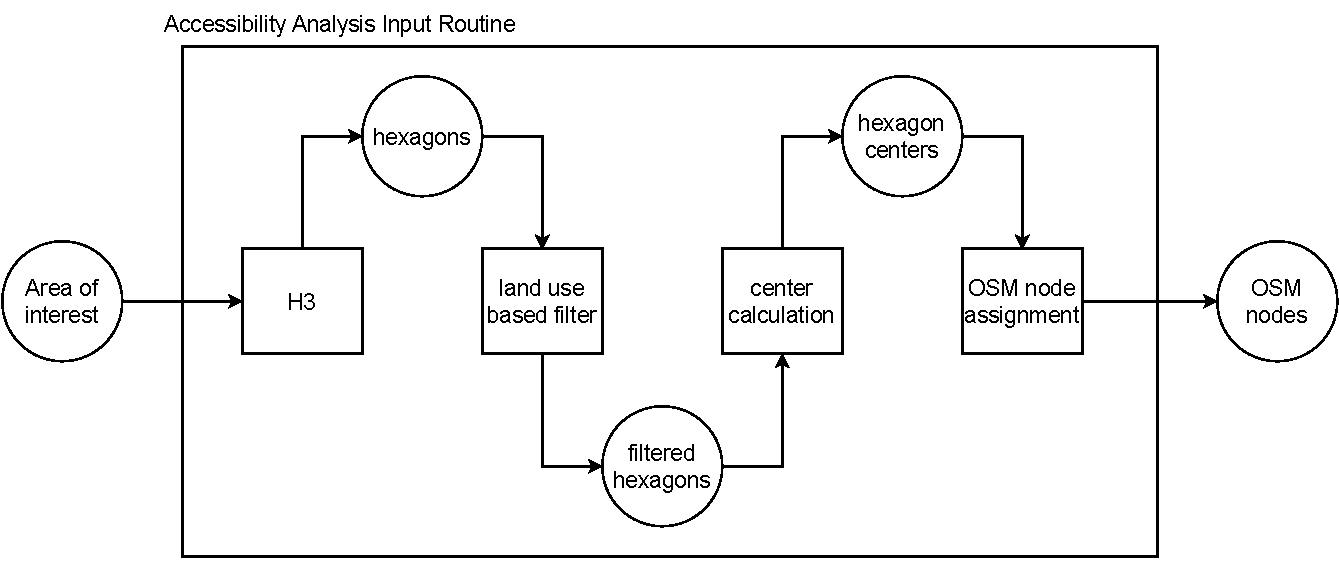
\includegraphics[scale=0.60]{Figures/method/input_routine}
    \caption{Input Routine}
    \label{fig:input_routine}
\end{figure}
In the input routine, depicted in Figure \ref{fig:input_routine}, we first create an even grid that covers the whole area of interest, for example a city.
To create such a grid, we use H3 \shortcite{H3H3}, which uses hexagons to evenly discretize an area.
Our goal will be to calculate our metric for each hexagon, so that we get detailed spatial information about the accessibility in the area of interest.
The chosen H3 resolution determines the size of these hexagons: a higher resolution means smaller hexagons, enhancing the granularity of our analysis. 
As such, selecting an appropriate H3 resolution is pivotal as it allows us to calculate our metrics for each hexagon with increased spatial accuracy, yielding a detailed spatial dataset that reflects the accessibility variations within the area of interest.
We recommend a resolution of nine, which corresponds to a hexagon edge length of roughly 200 meters, as it is a good compromise between accuracy and computation time.
The input routine also filters out uninteresting hexagons.
For, example we filter out hexagons that don't contain any residential areas, as there are no people living there is no need to access any amenities.
Next the input routine retrieves the centroid of each hexagon and then calculates the Euclidean distance between the centroids and the OSM nodes in order to assign the closest OSM node to each centroid.
The result of the input routine is a set of OSM nodes, for which we want to compute the accessibility.


% Main routine
\begin{figure}
    \centering
    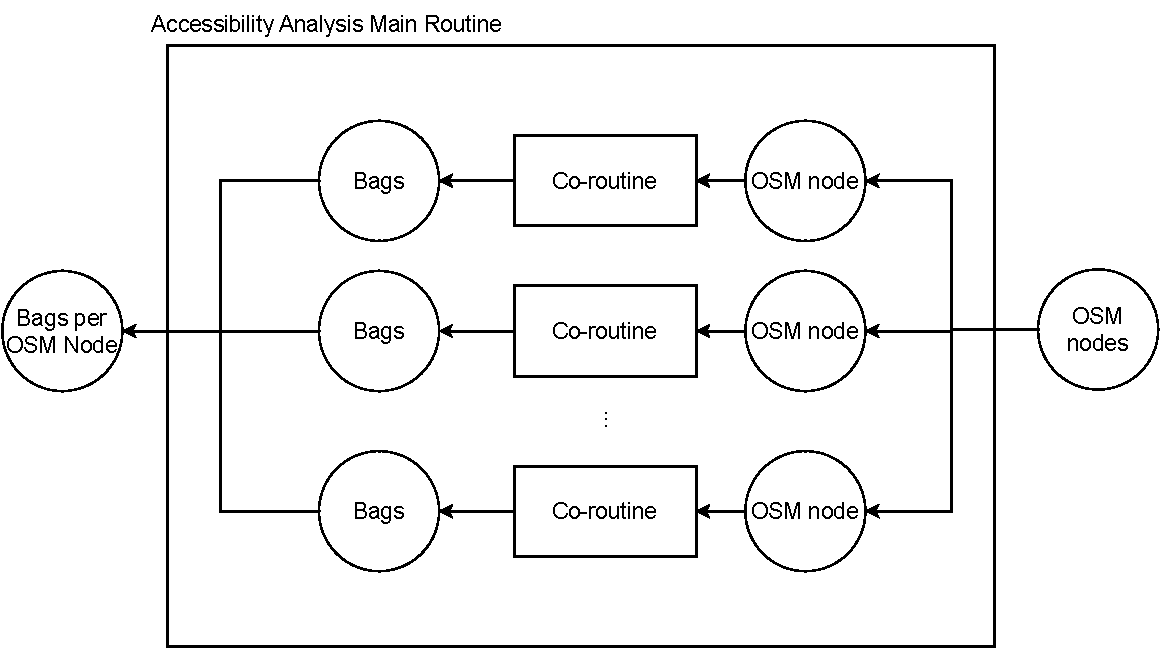
\includegraphics[scale=0.75]{Figures/method/main_routine}
    \caption{Main Routine}
    \label{fig:main_routine}
\end{figure}
The main routine, depicted in Figure \ref{fig:main_routine}, calls our scaffolding routing algorithm described in Section \ref{subsec:routing_algorithms} on each OSM node provided by the input routine.
This results in a set of Bags for each node.

% Metrics routine
\begin{figure}
    \centering
    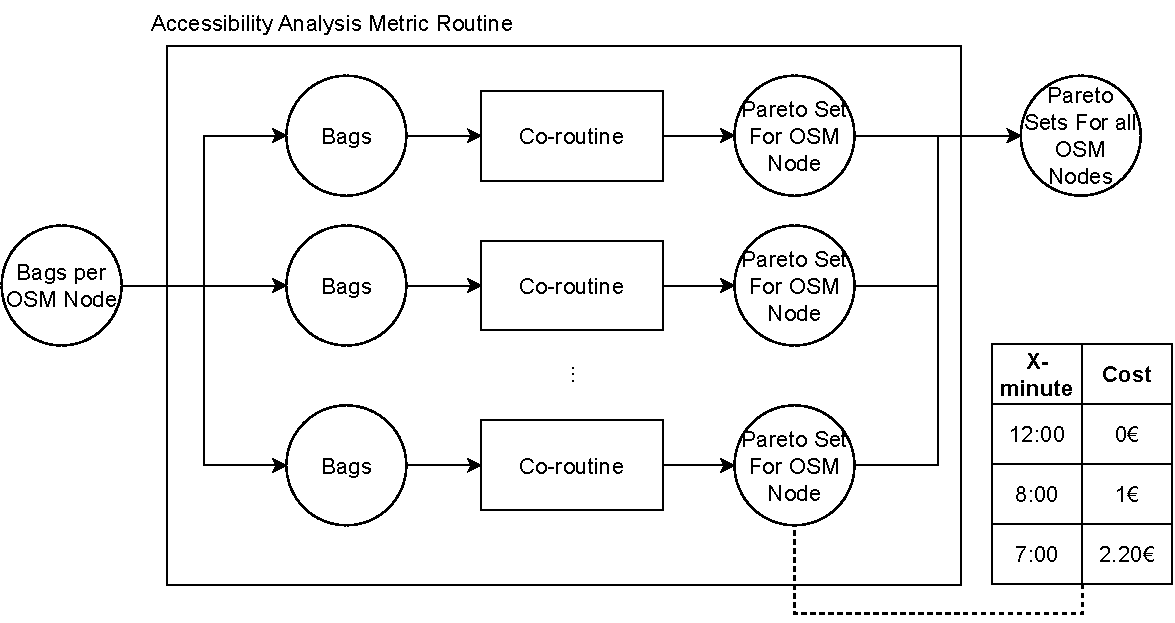
\includegraphics[scale=0.75]{Figures/method/metric_routine}
    \caption{Metric Routine}
    \label{fig:metric_routine}
\end{figure}
The metrics routine, depicted in Figure \ref{fig:metric_routine}, processes the bags into Pareto sets, where one entry in the Pareto set is a tuple of the X-minute city metric and the related cost.
To do so, we process each collection of bags separately - one co-routine for each OSM node/collection of bags.

\begin{figure}
    \centering
    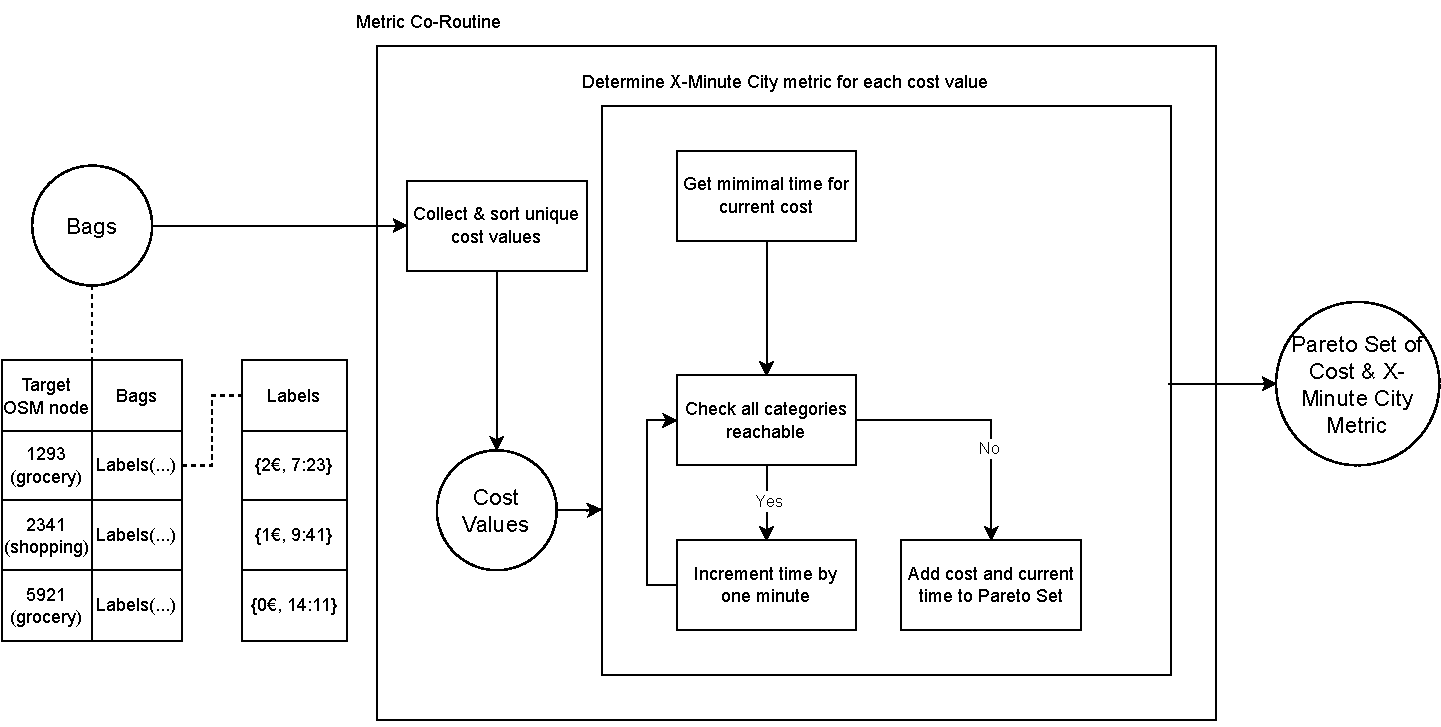
\includegraphics[scale=0.50]{Figures/method/metric_coroutine}
    \caption{Metric Co-Routine}
    \label{fig:metric_co_routine}
\end{figure}
The co-routine is depicted in Figure \ref{fig:metric_co_routine} and works as follows.
We start by collecting all unique cost values in each label in each bag and then sort them in ascending order.
For each cost value we then determine the associated X-minute city metric.
We do so by checking whether every category is reachable given the cost value and an iteratively increasing time value.
We start with a time value that is equal to the minimum time across all labels.
If all categories are reachable, we've found the X-minute city metric, which together with the cost value is added to the Pareto set.
If not, we increase the time value by one minute and check again.
We repeat this until all cost values are processed.
The result is a Pareto set for each OSM node/collection of bags.
